\subsection{统一时刻的径向误差剖面与角向误差谱}
\label{sec:review-profiles}

资格表中的各项最大误差不一定发生于同一时刻、网格或参考。为此，我们重新分析与已合格 GPU 轨迹绑定的高分辨率 CPU 控制：RFM41（种子 7331）、Legendre36 与 FD184。前两者使用原来的 $t_s=8$ 换步方案，非零模态均保留秩 40；恒步 RFM41 与 Legendre36 也纳入机器可读结果。参考仍为已有的 FD448/$K=144$ 轨迹：\texttt{angular\_fine} 的时间率为 384，\texttt{time\_fine} 为 512。本项分析不积分任何新参考或新候选。数据保留全部 19 个物理时刻，图中使用统一的 $8,24,48,72$ 时刻及 \texttt{time\_fine} 参考，不作相位对齐。

记速度向量或标量涡量的误差为 $e_f$，角向平均为 $\langle\cdot\rangle_\theta$。在原有 layer144 径向节点及物理面积权重 $w_i$ 上，定义
\begin{equation}
R_f^2=\frac{\sum_i w_i\langle|f_{\rm ref}(r_i,\cdot)|^2\rangle_\theta}{\sum_i w_i},
 \qquad P_f(r_i)=\frac{\langle|e_f(r_i,\cdot)|^2\rangle_\theta^{1/2}}{R_f}.
\label{eq:review-profile-norm}
\end{equation}

这一归一化避免了除以局部趋零的场值。实场采用非负 Fourier 模态表示时，角向误差贡献为
\begin{equation}
Q_{f,k}=\left(\frac{c_k\sum_i w_i|\widehat e_{f,k}(r_i)|^2}
 {\sum_i w_i\langle|f_{\rm ref}(r_i,\cdot)|^2\rangle_\theta}\right)^{1/2},
 \qquad c_0=1,\quad c_k=2\;(k>0).
\label{eq:review-modal-error}
\end{equation}

速度项在极坐标表示 $(u_r,u_\theta)$ 下对两个分量的平方幅值求和。逐点正交变换到 Cartesian 分量不改变积分后的向量误差能量，但能量在角向模态之间的分配依赖分量表示，因此图中速度谱明确是极坐标分量谱。$P_f^2$ 的加权平均和 $Q_{f,k}^2$ 的模态求和均等于相对场误差的平方。精确角向 Parseval 计算与原 layer144 物理网格打分在 380 项检查中的最大差为 $2.13\times10^{-17}$。超过候选截止频率 $K=80$ 的谱段是共同未解析的参考尾部，并非候选多出的自由度。

\begin{figure}[htbp]
\centering
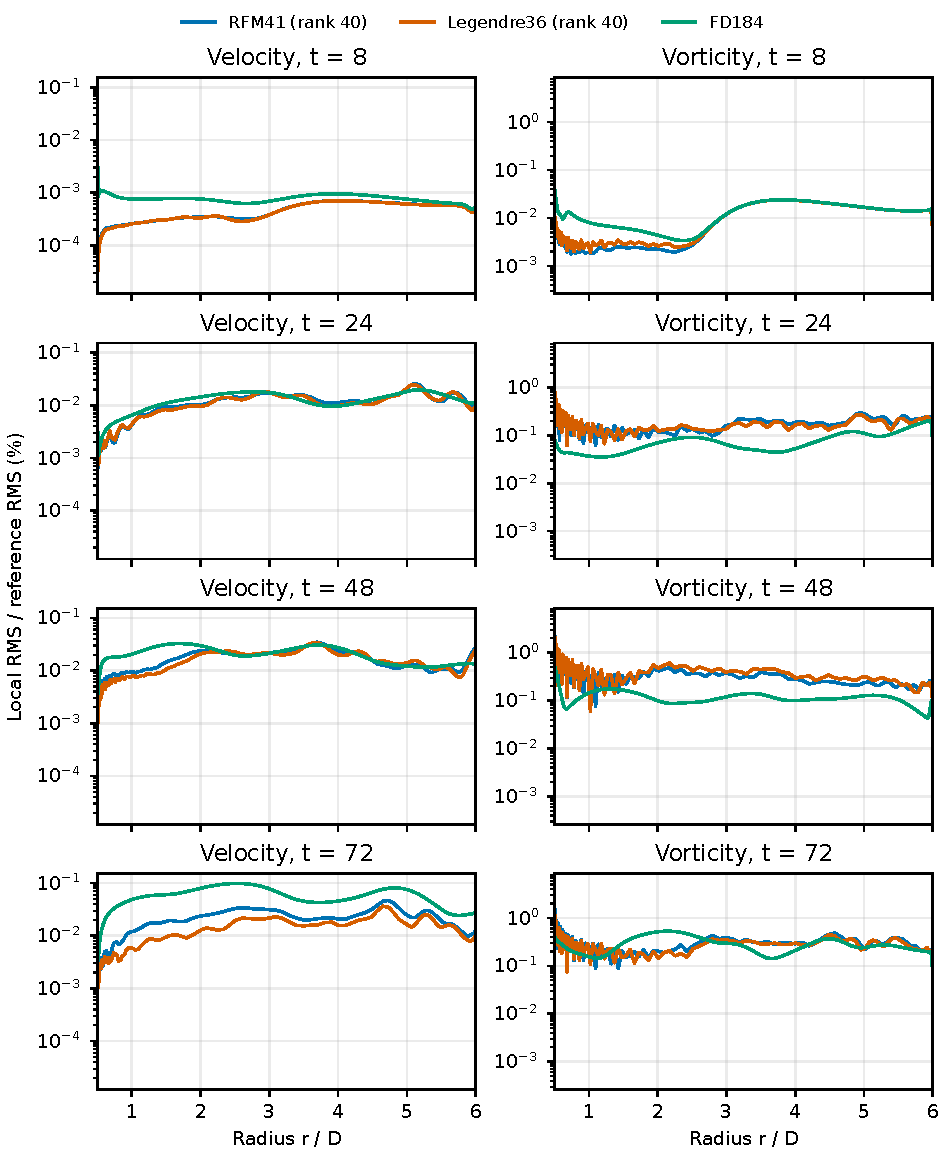
\includegraphics[width=\linewidth]{figures/review_radial_errors.pdf}
\caption{相对于已有时间细化参考的统一时刻径向误差剖面 $100P_f$。RFM41 使用种子 7331；Galerkin 曲线采用 $t_s=8$ 换步，FD184 保留已合格的时间方案。各面板内所有曲线具有相同的参考与时刻。纵轴为局部角向 RMS 误差除以全域参考 RMS，而非逐点相对误差。}
\label{fig:review-radial-errors}
\end{figure}

\begin{figure}[htbp]
\centering
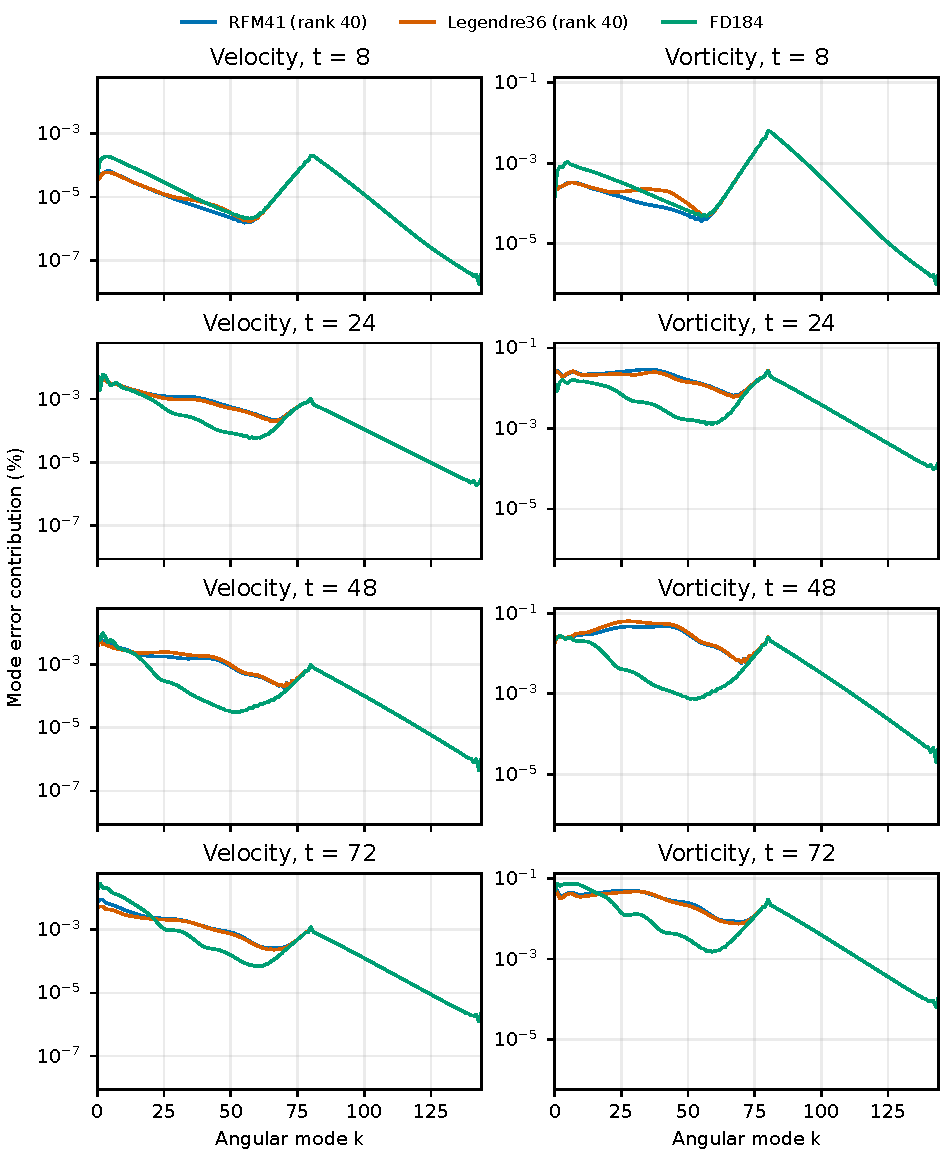
\includegraphics[width=\linewidth]{figures/review_angular_errors.pdf}
\caption{与图~\ref{fig:review-radial-errors} 相同轨迹和时刻的角向误差贡献 $100Q_{f,k}$。各模态贡献按平方和合成，并非逐模态独立归一化的误差。模态 80 以上的共同尾部来自更细参考的谱。}
\label{fig:review-angular-errors}
\end{figure}

原来的最大值不是同一流态下的排序。对本项 RFM 种子，全域速度与涡量最大误差分别出现在 $t=72$ 与 $60$；Legendre 对应最大值出现在 $60$ 与 $54$。改为统一的 $t=48$、layer144 网格后，RFM41、Legendre36、FD184 的速度误差分别为 $0.01886\%$、$0.01842\%$、$0.02053\%$，涡量误差却分别为 $0.29438\%$、$0.35509\%$、$0.11317\%$。因此，即使在同一时刻，速度误差排序仍不决定涡量误差排序。旋度依赖速度的一阶导数，仅比较速度的 $L^2$ 误差不足以控制导数误差。测得的谱与此相符：在 $t=72$，FD184 的速度平方误差范数中 $84.24\%$ 来自 $k\le8$；RFM41 的涡量平方误差范数中 $47.72\%$ 来自 $25\le k\le80$，而 FD184 对应比例为 $5.45\%$。

径向归因同样需要限定。在 $t=72$，RFM41 的涡量平方误差范数有 $61.14\%$ 位于 $r\ge4$，但只有 $1.37\%$ 位于 $r\ge5.9$，因此不能把观察到的误差描述为仅局限于极薄的最外层。这些诊断定位的是完整演化解中的误差，不能单独识别边界层基函数的因果收益，也不能分离径向逼近、时间离散、边界处理和参考不确定性。基函数归因需要配套的受控消融；仅凭本节图像不能得出这一结论。

\subsection{将切换时刻移至 $t_s=12$ 的 CPU 敏感性实验}
\label{sec:review-switch}

第三版修订实际新增四条积分至 $T=72$ 的 CPU 轨迹：时间率 $128\to112$ 的 RFM37 与 Legendre35，以及 $152\to136$ 的 RFM41 与 Legendre36，切换时刻由 8 改为 12。RFM 使用种子 7331，确定性对照保留原配置。现有 CPU 分段时钟已经接受显式切换时刻，但默认观测列表包含原 $t_s=8$ 的桥接检查点，因此独立驱动显式传入相同的 19 个物理时刻。底层求解器及归档数据没有改动。四个 worker 各使用一个 BLAS 线程，并行运行时间不作为隔离性能证据。恒步与 $t_s=8$ 使用已有 CPU 控制，不重复计算，也不计为新增实验。

四条新轨迹在保存的 $t\le12$ 时刻均与对应恒步 CPU 状态逐元素完全一致。全域及近场的速度、涡量在三个网格、两个冻结参考上均通过 $0.5\%$ 门槛；相对于对应恒步控制的逐格三角上界同样通过，探针交替变号持续存在。表~\ref{tab:review-switch12} 区分全域场最大误差与四个指标中最坏的上界。这是单个 RFM 种子的敏感性结果，不能当作新的五种子 GPU 资格实验。

\begin{table}[htbp]
\centering\small
\begin{tabular}{llrrrr}
\hline
配置 & 时间方案 & $E_u$ (\%) & $E_\omega$ (\%) & 上界 (\%) & $N_{\rm nl}$\\
\hline
RFM37 & 恒步 & 0.029428 & 0.409349 & 0.409349 & 9215\\
 & $t_s=8$ & 0.044672 & 0.431680 & 0.478647 & 8191\\
 & $t_s=12$ & 0.043821 & 0.429910 & 0.474465 & 8255\\
Legendre35 & 恒步 & 0.026763 & 0.442065 & 0.442065 & 9215\\
 & $t_s=8$ & 0.041043 & 0.456649 & 0.497730 & 8191\\
 & $t_s=12$ & 0.040211 & 0.455435 & 0.493773 & 8255\\
RFM41 & 恒步 & 0.018192 & 0.331380 & 0.331380 & 10943\\
 & $t_s=8$ & 0.025948 & 0.339890 & 0.368159 & 9919\\
 & $t_s=12$ & 0.025496 & 0.339258 & 0.365822 & 9983\\
Legendre36 & 恒步 & 0.016132 & 0.362049 & 0.362049 & 10943\\
 & $t_s=8$ & 0.019717 & 0.366338 & 0.394046 & 9919\\
 & $t_s=12$ & 0.019410 & 0.365962 & 0.391767 & 9983\\
\hline
\end{tabular}
\caption{冻结空间配置下的 CPU 切换时刻敏感性。误差在两个参考、三个网格及 19 个统一时刻上分别取最大值，每项指标有各自的最大值位置；上界还包含近场指标。RFM 行使用种子 7331，因此不必等于前文五种子最大值。$N_{\rm nl}$ 为实际非线性评估次数，推进 FFT 批次数为 $2N_{\rm nl}$。 $t_s=12$ 尚无GPU轨迹，因此这些行不附加CPU--GPU偏差界。}
\label{tab:review-switch12}
\end{table}

切换时刻由 8 移至 12 后，每种配置均增加 64 次非线性评估、128 个 FFT 批次；相对于恒步仍减少 960 次评估，中、高档分别节省 $10.418\%$ 与 $8.773\%$，而在 8 切换时分别节省 $11.112\%$ 与 $9.358\%$。误差改善幅度较小：RFM37 的速度最大值降低 $0.000851$ 个百分点，涡量最大值降低 $0.001771$ 个百分点。新结果中最接近门槛的上界为 Legendre35 的 $0.493773\%$。因此，后移切换在本算例中以少量额外工作换得少量精度余量，不能据此给出隔离速度排名。

横向触发脉冲在 $t=12$ 终止，其 $\sin^4$ 形状在该连接点为 $C^3$，四阶导数可能跳跃。因此，桥接局部 Taylor 一致性推导必须尊重连接点实际具有的单侧正则性。本项是切换时刻敏感性实验，不能称为消除了平滑瞬态的降阶；本次也未提供用于估计观测阶数的时间步细化序列。此外，归档的 $10^{-5}$ 实现门槛比较的是\emph{同一离散时间方案}的 CPU/GPU 或 CPU 算子实现，不是允许改变恒步与分段时间离散的容差；后者由物理误差及 $0.5\%$ 三角上界评价。审稿引用的中档 RFM 速度最大值 $0.029428\%$ 与 $0.044672\%$ 相差 $0.015244$ 个百分点，相对增幅约 $51.8\%$；核对后两项恰好均在 $t=72$。仅凭这一相对增幅，无法确认瞬态分裂机制或阶数降低。

\paragraph{范数降低不等于因果误差分摊。}
对中档RFM的速度最大误差而言，延后换步恢复了相对恒步增量的约 $5.584\%$。这只是算术比值 $(E_8-E_{12})/(E_8-E_U)$，并未隔离桥接单步的误差。该干预同时改变了四个时间单位内的细步/粗步积分、桥接时刻与状态，以及后续误差历史。且 $t=8$ 位于解析脉冲内部，不是非光滑激励拼接点。

保存流场可直接说明非可加性。令 $e_8=u_8-u_{\rm ref}$、$e_{12}=u_{12}-u_{\rm ref}$、$\delta=e_8-e_{12}$，统一使用物理面积内积，并除以 $\|u_{\rm ref}\|^2$，则
\begin{equation}
 \|e_8\|_{\rm ref}^2=\|e_{12}\|_{\rm ref}^2+
 2\langle e_{12},\delta\rangle_{\rm ref}+\|\delta\|_{\rm ref}^2.
 \label{eq:review-switch-attribution}
\end{equation}
对RFM37种子7331，取 $t=72$、layer144网格及时间细化参考，四项依次为 $1.9956194141\times10^{-7}$、$1.9202943907\times10^{-7}$、$7.4475738974\times10^{-9}$、$8.4928450335\times10^{-11}$，均为未乘百分比尺度的相对误差平方。未舍入恒等式残差为 $2.04\times10^{-22}$；交叉项约占平方范数差的 $98.87\%$。这条确定性恒等式说明，$5.6\%$ 的恢复比例及其 $94.4\%$ 补数都不是独立的物理误差成分。若要因果区分桥接与后续粗步误差，仍需单独控制相应干预并做时间步细化研究。

